\documentclass[a0paper,portrait]{baposter}
%%%%%%%%%%%%%%%%%%%%%%%%%%%%%%%%%%%%%%%%%%%%%%%%
% Language, Encoding and Fonts
% http://en.wikibooks.org/wiki/LaTeX/Internationalization
%%%%%%%%%%%%%%%%%%%%%%%%%%%%%%%%%%%%%%%%%%%%%%%%
% Select encoding of your inputs. Depends on
% your operating system and its default input
% encoding. Typically, you should use
%   Linux  : utf8 (most modern Linux distributions)
%            latin1 
%   Windows: ansinew
%            latin1 (works in most cases)
%   Mac    : applemac
% Notice that you can manually change the input
% encoding of your files by selecting "save as"
% an select the desired input encoding. 
\usepackage[utf8]{inputenc}
% Make latex understand and use the typographic
% rules of the language used in the document.
\usepackage[english]{babel}
% Use the vector font Latin Modern which is going
% to be the default font in latex in the future.
\usepackage{helvet}
% Change the default font family from roman to sans serif
\renewcommand{\familydefault}{\sfdefault} % for text
\usepackage[helvet]{sfmath} % for math
% Choose the font encoding
\usepackage[T1]{fontenc}
\usepackage{makecell}
\usepackage{auto-pst-pdf}
\usepackage{pst-pdf}
\usepackage{pst-coil}

%%%%%%%%%%%%%%%%%%%%%%%%%%%%%%%%%%%%%%%%%%%%%%%%
% Graphics and Tables
% http://en.wikibooks.org/wiki/LaTeX/Importing_Graphics
% http://en.wikibooks.org/wiki/LaTeX/Tables
% http://pgfplots.sourceforge.net/
%%%%%%%%%%%%%%%%%%%%%%%%%%%%%%%%%%%%%%%%%%%%%%%%
% You cannot use floats in the baposter theme.
% We therefore load the caption package which provides
% the command \captionof
% Set up how figure and table captions are displayed
\usepackage{caption}
\captionsetup{
  font=small,% set font size to footnotesize
  labelfont=bf % bold label (e.g., Figure 3.2) font
}
% Make the standard latex tables look so much better
\usepackage{array,booktabs}
% For creating beautiful plots
\usepackage{pgfplots}

%%%%%%%%%%%%%%%%%%%%%%%%%%%%%%%%%%%%%%%%%%%%%%%%
% Mathematics
% http://en.wikibooks.org/wiki/LaTeX/Mathematics
%%%%%%%%%%%%%%%%%%%%%%%%%%%%%%%%%%%%%%%%%%%%%%%%
% Defines new environments such as equation,
% align and split 
\usepackage{amsmath}
% Adds new math symbols
\usepackage{amssymb}

%%%%%%%%%%%%%%%%%%%%%%%%%%%%%%%%%%%%%%%%%%%%%%%%
% Colours
% http://en.wikibooks.org/wiki/LaTeX/Colors
%%%%%%%%%%%%%%%%%%%%%%%%%%%%%%%%%%%%%%%%%%%%%%%%
\selectcolormodel{RGB}
% define the three aau colors
\definecolor{aaublue1}{RGB}{33,26,82}% dark blue
\definecolor{aaublue2}{RGB}{113,109,143} % light blue
\definecolor{aaublue3}{RGB}{194,193,204} % lighter blue

%%%%%%%%%%%%%%%%%%%%%%%%%%%%%%%%%%%%%%%%%%%%%%%%
% Lists
% http://en.wikibooks.org/wiki/LaTeX/List_Structures
%%%%%%%%%%%%%%%%%%%%%%%%%%%%%%%%%%%%%%%%%%%%%%%%
% Easier configuration of lists
\usepackage{enumitem}
%configure itemize
\setlist{%
  topsep=0pt,% set space before and after list
  noitemsep,% remove space between items
  labelindent=\parindent,% set the label indentation to the paragraph indentation
  leftmargin=*,% remove the left margin
  font=\color{aaublue1}\normalfont, %set the colour of all bullets, numbers and descriptions to aaublue1
}
% use set<itemize,enumerate,description> if you have an older latex distribution
\setitemize[1]{label={\raise1.25pt\hbox{$\blacktriangleright$}}}
\setitemize[2]{label={\scriptsize\raise1.25pt\hbox{$\blacktriangleright$}}}
\setitemize[3]{label={\raise1.25pt\hbox{$\star$}}}
\setitemize[4]{label={-}}
%\setenumerate[1]{label={\theenumi.}}
%\setenumerate[2]{label={(\theenumii)}}
%\setenumerate[3]{label={\theenumiii.}}
%\setenumerate[4]{label={\theenumiv.}}
%\setdescription{font=\color{aaublue1}\normalfont\bfseries}

% use setlist[<itemize,enumerate,description>,<level>] if you have a newer latex distribution
%\setlist[itemize,1]{label={\raise1.25pt\hbox{$\blacktriangleright$}}}
%\setlist[itemize,2]{label={\scriptsize\raise1.25pt\hbox{$\blacktriangleright$}}}
%\setlist[itemize,3]{label={\raise1.25pt\hbox{$\star$}}}
%\setlist[itemize,4]{label={-}}
%\setlist[enumerate,1]{label={\theenumi.}}
%\setlist[enumerate,2]{label={(\theenumii)}}
%\setlist[enumerate,3]{label={\theenumiii.}}
%\setlist[enumerate,4]{label={\theenumiv.}}
%\setlist[description]{font=\color{aaublue1}\normalfont\bfseries}

%%%%%%%%%%%%%%%%%%%%%%%%%%%%%%%%%%%%%%%%%%%%%%%%
% Misc
%%%%%%%%%%%%%%%%%%%%%%%%%%%%%%%%%%%%%%%%%%%%%%%%
% change/remove some names
\addto{\captionsenglish}{
  %remove the title of the bibliograhpy
  \renewcommand{\refname}{\vspace{-0.7em}}
  %change Figure to Fig. in figure captions
  \renewcommand{\figurename}{Fig.}
}
% create links
\usepackage{url}
%note that the hyperref package is currently incompatible with the baposter class

%%%%%%%%%%%%%%%%%%%%%%%%%%%%%%%%%%%%%%%%%%%%%%%%
% Macros
%%%%%%%%%%%%%%%%%%%%%%%%%%%%%%%%%%%%%%%%%%%%%%%%
\newcommand{\alert}[1]{{\color{aaublue1}#1}}

%%%%%%%%%%%%%%%%%%%%%%%%%%%%%%%%%%%%%%%%%%%%%%%%
% Document Start 
%%%%%%%%%%%%%%%%%%%%%%%%%%%%%%%%%%%%%%%%%%%%%%%%
\begin{document}
%%%%%%%%%%%%%%%%%%%%%%%%%%%%%%%%%%%%%%%%%%%%%%%%
% Some changes that cannot be made in the preamble
%%%%%%%%%%%%%%%%%%%%%%%%%%%%%%%%%%%%%%%%%%%%%%%%
% set the background of the poster
\background{
  \begin{tikzpicture}[remember picture,overlay]%
    %the poster background color
    \fill[fill=aaublue3] (current page.north west) rectangle (current page.south east);
    %the header
    \fill [fill=aaublue1] (current page.north west) rectangle ([yshift=-\headerheight] current page.north east);
  \end{tikzpicture}
}
% if you want to reduce the space before and after equations, use and adjust
% the following lines
%\addtolength{\abovedisplayskip}{-2mm}
%\addtolength{\belowdisplayskip}{-2mm}

%%%%%%%%%%%%%%%%%%%%%%%%%%%%%%%%%%%%%%%%%%%%%%%%
% General poster setup
%%%%%%%%%%%%%%%%%%%%%%%%%%%%%%%%%%%%%%%%%%%%%%%%
\begin{poster}{
  %general options for the poster
  grid=false,
  columns=3,
%  colspacing=4.2mm,
  headerheight=0.2\textheight,
  background=user,
%  bgColorOne=red!42, %is used when background != user and none
%  bgColortwo=green!42, %is used when background is shaded
  eyecatcher=true,
  %posterbox options
  headerborder=closed,
  borderColor=aaublue1,
  headershape=rectangle,
  headershade=plain,
  headerColorOne=aaublue1,
%  headerColortwo=yellow!42, %is used when the header background is shaded
  textborder=rectangle,
  boxshade=plain,
  boxColorOne=white,
%  boxColorTwo=cyan!42,%is used when the text background is shaded
  headerFontColor=white,
  headerfont=\Large\sf\bf,
  linewidth=1pt
}
%the Eye Catcher (the logo on the left)
{
  %this can be commented out or replaced by a company/department logo
  
\includegraphics[height=0.2\headerheight]{AAUgraphics/aau_logo_new_neg}
}
%the poster title
{\color{white}\bf
\huge
    Graph Based Physical Models for Sound Synthesis 
}
%the author(s)
{\color{white}\small
  \vspace{1em}
    \begin{tabular}[t]{c c}
        \raisebox{-\height+\baselineskip}{\makecell
        {
            \small
            Pelle Juul Christensen\\[0.5em] \\
            Aalborg University Copenhagen, Denmark\\
            pelle.juul@tuta.io
        }} &
        \raisebox{-\height+\baselineskip}{\makecell
        {
            \small
            Stefania Serafin\\[0.5em]
            Multisensory Experience Lab \\ Aalborg University Copenhagen, Denmark\\
            sts@create.aau.dk
        }}
    
    \end{tabular}
}
%the logo (the logo on the right)
{
  %this can be commented out or replaced by a company/department logo
  
\includegraphics[height=0.2\headerheight]{AAUgraphics/aau_logo_new_neg}
}

%%%%%%%%%%%%%%%%%%%%%%%%%%%%%%%%%%%%%%%%%%%%%%%%
% the actual content of the poster begins here
%%%%%%%%%%%%%%%%%%%%%%%%%%%%%%%%%%%%%%%%%%%%%%%%

\begin{posterbox}[name=intro,column=0,row=0]{Introduction}

Recent research in physical models has been directed towards simulating systems using \textit{finite difference schemes}\cite{numericalSoundSynthesis}, which can be used to model the intricacies of many kinds of vibrating systems and exciters.

As many other physical modelling methods, finite difference schemes can be used to simulate systems which are hard to construct in real life.

Some research has explored this idea further by building abstract physical models that do not have any direct relation to any real world instruments. 

Our paper further explores the notions of abstract physical models by
showing a way of building systems of connected strings that would not necessarily be achievable or practical in real life.

\end{posterbox}

\begin{posterbox}[name=usage,column=0,below=intro]{Theory}
In order to derive the theory to build graph base physical models we start with the 1D wave equation and move on the a branching topology.
    
The 1D wave equation can be derived by considering a string of connected masses as in Fig. \ref{fig:springLine}.  
\begin{center}
    \psscalebox{0.8 0.8}
    {
        \input{figures/spring-line}
    }
    \captionof{figure}{A section of a line topology string viewed as a lumped mass-spring network.}
    \label{fig:springLine}
\end{center}

The dynamics of mass $u_l$ is determined by the differential equation
\begin{equation}
    \label{eq:linePhys}
    \frac{d^2u_l}{dt^2} = \frac{E}{\rho}\left(\frac{u_{l+1} - 2u_{l} + u_{l-1}}{h^2} \right).
\end{equation}
If we select $c = \sqrt{E / \rho}$ the right hand side of Equation
(\label{eq:linePhys}) is equal to the right hand side of the dicretized 1D
wave equation
\begin{equation}
    \label{eq:discretized1dWave}
    \delta_{tt} u^{n}_{l} = c^2 \delta_{xx} u^{n}_{l},
\end{equation}
where the difference operators are defined as
\begin{alignat}{2}
\delta_{tt} u^n_l &= \frac{1}{k^2}(u^{n+1}_l - 2u^n_l + u^{n-1}_l)   &&\approx \frac{d^2u}{dt^2}, \\
\label{eq:secondOrderDiff}
\delta_{xx} u^{n}_{l} &= \frac{1}{h^2}(u^{n}_{l+1} - 2u^{n}_{ l} + u^{n}_{ l+1}) &&\approx \frac{d^2u}{dt^2}.
\end{alignat}
\vfill
\end{posterbox}

\begin{posterbox}[name=theory2,column=1]{Theory --- Continued}
Now we perform the same derivation, but for the branching topology shown in Fig. \ref{fig:springBranch}.
\begin{center}
    \psscalebox{0.8 0.8}
    {
        \input{figures/spring-branch}
    }
    \captionof{figure}{The branching point of a branching topology viewed as a mass-spring network.} 
    \label{fig:springBranch}
\end{center}
The dynamics of mass $u_l$ is now determined by the differential equation
\begin{equation}
    \frac{d^2u_L}{dt^2} = \frac{E}{\rho}\left(\frac{\overset{1}{u}_{1} + \overset{2}{u}_{1} + u_{L-1} - 3u_{L}}{h^2} \right),
\end{equation}
From which we get the definition
\begin{equation}
    \delta_{xx}u_L = \frac{1}{h^2}(\overset{1}{u}_{1} + \overset{2}{u}_{1} + u_{L-1} - 3u_{L}).
\end{equation}

We can generalize this to an N-branch topology like in Fig.  \ref{fig:graphNbranch}.

\begin{center}
    \psscalebox{1.2 1.2}
    {
        \input{figures/graph-nbranch}
    }
    \captionof{figure}{A model with an $N$-branch topology.}
    \label{fig:graphNbranch}
\end{center}

In this case we get a definition for the second order spatial difference operator which looks like:

\begin{equation}
    \label{eq:dxxBranch}
    \delta_{\Delta\mathbb{U}}u_l = \frac{1}{h^2}\left(\sum_{\overset{*}{u} \in
    \mathbb{U}_l} \overset{*}{u} - |\mathbb{U}_l| u_l\right),
\end{equation}

which we can then use to construct any possible graph topology.

\end{posterbox}

\begin{posterbox}[name=buildinggraphs,column=1,below=theory2]{Building Graphs}
Using Equation (\ref{eq:dxxBranch}) we can build any graph. Some archetypes
can be seen in Fig. \ref{fig:graphTree}.

    \begin{center}
    \begin{tabular}{c c c}
        \makecell{
            a)\\
            \psscalebox{0.8 0.8}{\input{figures/graph-tree}}
        } &
        \makecell{
            b)\\
            \psscalebox{0.8 0.8}{\input{figures/graphLoop}}} &
        \makecell{
            c)\\
            \psscalebox{0.8 0.8}{\input{figures/graphCycle}}}
    \end{tabular}
        \captionof{figure}{Various graph topologies. a) A binary tree topology
        with multiple layers. b) A simple cyclic graph. c) A string connected to
        itself.}
        \label{fig:graphTree}
    \end{center}
\end{posterbox}

\begin{posterbox}[name=dense,column=2]{Dense Topologies}
    If we build a model mostly strings of length one we call it dense. E.g. a rectangular grid as seen in Fig.
    \ref{fig:tightGrid}.

    \begin{center}
        \psscalebox{0.8 0.8}{\input{figures/tightGrid.ps.py}}
        \captionof{figure}{A dense rectangular grid. The zigzag lines, symbolising springs,
            are drawn to show that the model has no internal strings.}
        \label{fig:tightGrid}
    \end{center}

    Alternatively a hexagonal grid, which has better performance than the
    rectangular grid, as in Fig. \ref{fig:hexGrid}.

    \begin{center}
        \psscalebox{0.5 0.5}{\input{figures/hexGrid.ps.py}}
        \captionof{figure}{A dense hexagon grid.} 
        \label{fig:hexGrid}
    \end{center}

    Note that dense models do not need to be grids and that grids are not
    necessarily dense.

\end{posterbox}

\begin{posterbox}[name=other,column=2,below=dense]{Extensions and Other Findings}
\begin{itemize}
    \item We can fairly easily add Dirichlet and Neumann boundary conditions to
        a model.
    \item The worst case complexity for an acyclic model is $\mathcal{O}(n)$
        while the worst case for cyclic models is $\mathcal{O}(n^2)$
    \item The harmonic content of a model can be known beforehand by computing the
        eigen frequencies of the system.
    \item Graph models can also be applied to bars, stiff strings and other
        acoustical objects.
\end{itemize}
\end{posterbox}

\begin{posterbox}[name=implementation,column=2,below=other]{Implementation}
    A reference implementation in \textsc{matlab} is available as well as an
    interactive C++/JUCE app.
    \begin{center}
        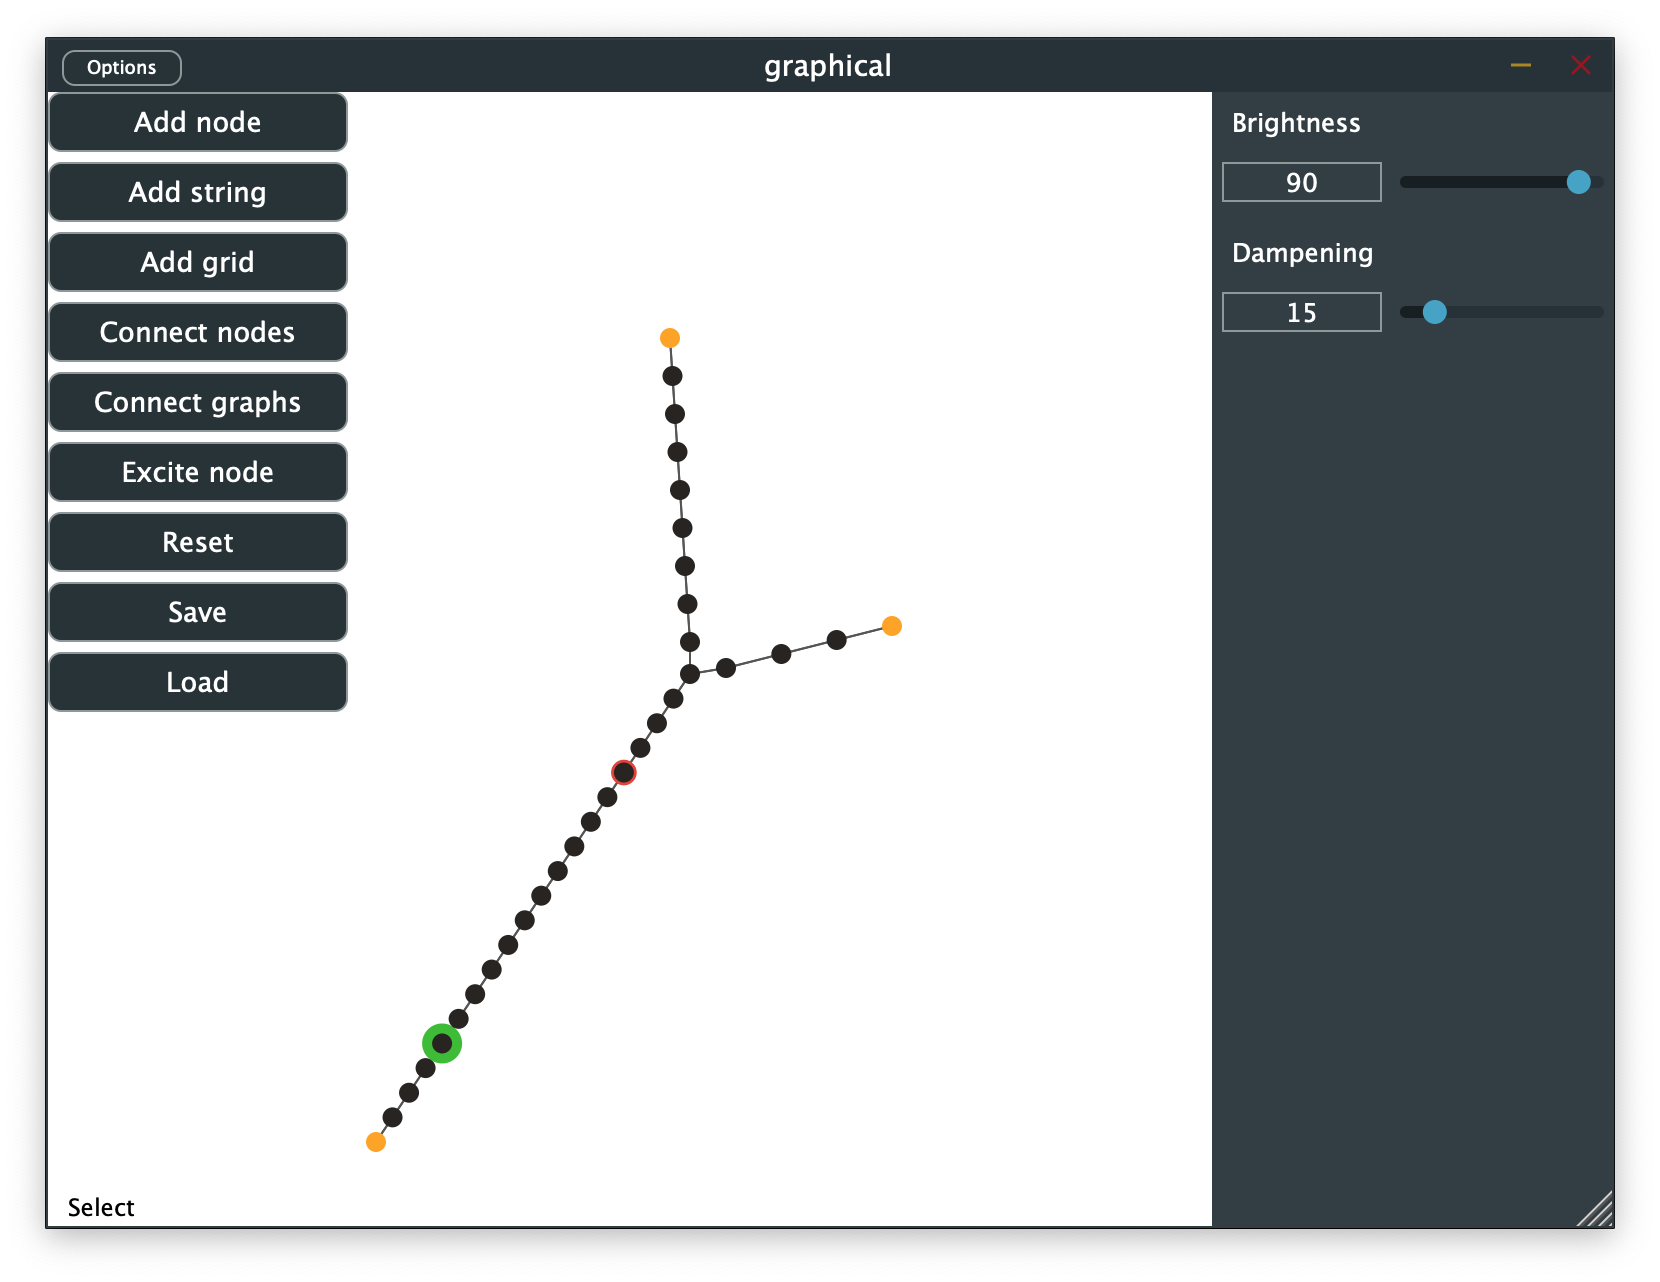
\includegraphics[width=0.8\textwidth]{gui.png}
        \captionof{figure}{Screen shot of the GUI C++/JUCE application.}
    \end{center}
\end{posterbox}
\end{poster}
\end{document}
